% !TeX spellcheck = en_US
\documentclass[letterpaper,12pt,twoside]{report}
\usepackage{fancyhdr}
\usepackage{fullpage}
\usepackage{tikz}
\usepackage{amsmath}
\usepackage{textcomp}

\begin{document}
	\pagestyle{fancy}
	\fancyhf{}
	\fancyhead[L]{Day 10}
	\fancyhead[R]{\textit{The Calendar Project}}
	\fancyfoot[L]{Citations Involved: ???}
	
	% Problem
	\paragraph{Problem}
	\begin{quote}
		\textsf{A circle of radius 1cm is inscribed in a right triangle. If one leg of the triangle has length of 3cm, find the length of the other leg.}
	\end{quote}
	
	% Graphics
	\begin{center}
		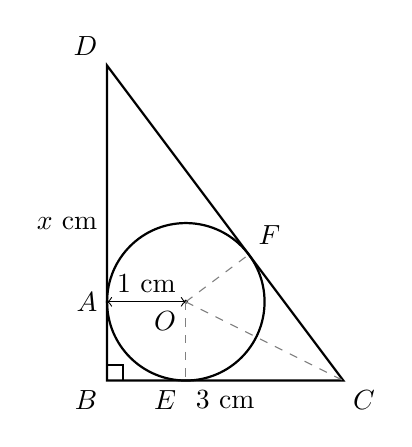
\begin{tikzpicture}[scale=1]
		\draw[thick] (0,0) circle [radius=1];
		\draw[thick] (-1,-1) -- (2,-1) -- (-1,3) -- cycle;
		\draw[thick] (-1,-0.8) -- (-0.8,-0.8) -- (-0.8,-1);
		\draw[fill=black] (0,0) circle [radius=0.02];
		\draw[<->] (0,0) -- (-1,0);
		
		\node[below left] at (0,0) {$O$};
		\node[below] at (0.5,-1) {$3$ cm};
		\node[left] at (-1,1) {$x$ cm};
		\node[above] at (-0.5,0) {$1$ cm};
		
		\node[left] at (-1,0) {$A$};
		\node[below left] at (-1,-1) {$B$};
		\node[below right] at (2,-1) {$C$};
		\node[above left] at (-1,3) {$D$};
		\node[below left] at (0,-1) {$E$};
		\node[above right] at (0.8,0.6) {$F$};
		
		\draw[dashed][gray] (0,0) -- (0,-1);
		\draw[dashed][gray] (0,0) -- (0.8,0.6);
		\draw[dashed][gray] (0,0) -- (2,-1);
		\end{tikzpicture}
	\end{center}
	
	% Reasoning
	\paragraph{Reasoning}
	\begin{quotation}
		
		$O$ is the center of the inscribed circle and is equidistant to $A$, $E$, and $F$; therefore $OA=OE=OF=1 \text{cm}$. Since an inscribed circle touches all sides of the shape it inscribes at exactly one point, it is tangent to the sides of the triangle. If a line is tangent to a circle, then it is perpendicular to the radius drawn to the point of tangency ($A$, $F$ and $E$); this means that $\overline{OA} \bot \overline{DB}$, $\overline{OF} \bot \overline{DC}$, and $\overline{OE} \bot \overline{BC}$. By the definition of perpendicular segments, $\angle OAB$, $\angle OEB$, and $\angle OFC$ are all right angles. With three right angles already known, quadrilateral $AOBE$ is proven to be a rectangle. With two adjacent sides congruent ($\overline{AO} \cong \overline{OE}$), it is additionally proven to be a square. Since all sides of a square are congruent by definition, $\overline{AO}\cong \overline{OE}\cong \overline{EB}\cong \overline{BA}$ and thus $AO=OE=EB=BA=1 \text{cm}$. $BC=EC+EB$ by the SAP, so $3=EC+1$ and thus $EC=2$. Since the trignometric ratio for tangent can be expressed as $\frac{\text{opposite}}{\text{adjacent}}$, $\tan \angle ECO = \frac{1}{2}$ and thus $\angle ECO=\arctan (\frac{1}{2}) \approx 26.565$\textdegree. Since $\overline{FC}$ and $\overline{EC}$ are both segments tangent to the inscribed circle with a common external endpoint $C$ (11-1-3), $\overline{EC}\cong \overline{FC}$; with this information, $\triangle ECO \cong \triangle FCO$ by the HL theorem, and $\angle ECO \cong \angle FCO$ by CPCTC. By the definition of angle congruence, $\text{m}\angle ECO = \text{m}\angle FCO = \arctan (\frac{1}{2}) $. By the Angle Addition Postulate, $\text{m}\angle ECO+\text{m}\angle FCO=\text{m}\angle ECF$. With substitution, this becomes $\arctan (\frac{1}{2}) + \arctan (\frac{1}{2}) = \text{m}\angle ECF=2\arctan (\frac{1}{2})$. Since $\triangle CBD$ is given to be a right triangle, $\tan \angle ECF = \frac{DB}{BC}$. Knowing that $BC=3$ and that $\angle ECF=2\arctan (\frac{1}{2})$, $DB=BC \tan (2 \arctan (\frac{1}{2}))=\frac{4}{3}BC=\frac{4}{3}(3)=\boxed{4 \text{cm}}$. 
		
	\end{quotation}
	
\end{document}